\clearpage
\chapter{Background}
\label{ch:background}
In this chapter, we review the precedent for contemporary explorations of
time and space in music. While far too many projects exist to cover
the all, we focus on projects that either particularly impactful, or
particularly relavant to the projects described in this thesis, noting
important details and differences whenever necessary. We conclude with
a deeper study of Iannis Xenakis' involvement in the 1958 Philips
Pavilion at the Brussels World Fair. This is particularly relevant in
that it made innovational use of sound and space, but stochastic
theory that connects the projects in this thesis. 

\paragraph{Early Spatial Music} Western spatial music emerged during
the renaissance period. The earliest published example of spatial
music was by Adrian Willaert in 1550.\cite{Zvonar1999} The Basilica
San Marco, in Venice, where Willaert was \textit{maestro di capella}
had an interesting feature: Two separate pipe organs facing each other
across the chapel. Willaert took advantage of the organs by composing
music for separate choirs and instrumental groups adjacent the two
organs. Spatially separate choirs soon became a fashion, and gradually
spread beyond Venice, as more and more spatially separated groups were
incorporated into composition. In honor of Queen Elizabeth's 40th
birthday in 1573, Thomas Tallis composed \textit{Spem in alium}, a
choral piece with 40 separate parts arranged in eight spatially
separated choirs. However, interest in spatial composition declined
toward the end of the Baroque period, and was largely avoided until
the Romantic period. Beriloz' \textit{Requiem} in 1837, Giuseppe
Verdi's \textit{Requiem} in 1874, and Mahler's \textit{Symphony No. 2}
in 1895 all feature spatially separated brass ensembles.

\paragraph{Tempo Acceleration and Deceleration}
Chapter \ref{ch:polytempic} \marginnote{Do not to confuse polytempic
  music with poly\textit{metric} and poly\textit{rhythmic}
  music. Polyrhythms and polymeters are common in West
  African musical tradition, and appear much earlier in Western music
  than polytempi.}  is concerned with oblique, similar, and contrary
tempo accelerations and decelerations in the context of polytempic
(with two or more simultaneous tempi) music.  The tempo indicators
commonly seen today such as \textit{allegro} and \textit{adagio} emerged
during the 17th century in Italy. While these markings partly express
a mood (\textit{gaily}, and \textit{with leisure} respectively) rather
than a strict tempo, they where much easier to follow than the
proportional system (based on tempic ratios such as 3:2 and 5:4) that
they replaced.\cite{Sachs1953} The intentional use of gradual tempo
changes likely evolved from the unconscious but musical tempo
fluctuations of a natural human performance. We can see examples of
the purposeful manipulation of tempo in the baroque
period. Monteverdi's \textit{Madrigali guerrieri} from 1638, includes
adjacent pieces: \textit{Non havea Febo ancora}, and \textit{Lamento
  della ninfa}. The score instructs to perform the former piece
\textit{al tempo della mano}, in the tactus of the conducting hand,
and the latter \textit{a tempo del'affetto del animo e non a quello
  della mano}, ``in a tempo [dictated by] emotion, not the hand.''
While Monteverdi's use of controlled tempo was certainly not the
first, we are (in particular) interested in gradual tempo changes in
polytempic compositions, which do not appear in western music until
near the beginning of the 20th century.

%\section{Wagner's Gessamtkunstwerk}

\section{20th Century Modernism}
\label{sec:modernism}
As the romantic period was coming to an end, there was a blossoming of
complexity, diversity, and invention in contemporary music. Performers
developed the virtuosic skills required to play the music, composers
also wrote increasingly difficult scores to challenge the
performers.\cite{Grout2006} Works by Italian composer Luciano Berio
illustrate the complexity of contemporary music of the time. Beginning
in 1958, Berio wrote a series of works he called
\textit{Sequenza}. Each was a highly of highly technical composition
written for a virtuosic soloist. Each was for a different instrument
ranging from flute to guitar to accordion.  In Sequenza~IV, for piano,
Berio juxtaposes thirty-second note quintuplets, sextuplets, and
septuplets (each with a different dynamic), over just a few
measures. 

\section{Polytempic Music}
\label{sec:background-polytempi}
Western polytempi can be traced Henry Cowell's book, \textit{New Musical
  Resources}, first published in 1930, wherein Cowell states:
\begin{quotation}
  ``Rhythm presents many interesting problems, few of which have been
  clearly formulated. Here, however, only one general idea will be
  dealt with-namely, that of the relationship of rhythm, which have an
  exact relationship to sound-vibration, and, through this
  relationship and the application of overtone ratios, the building of
  ordered systems of harmony and counterpoint in rhythm, which have an
  exact relationship to tonal harmony and
  counterpoint.''\sidenote{Examples from \textit{New Musical
      Resources} are from 3rd edition, published in
    1996.}\cite{Cowell1996}
\end{quotation}
Cowell goes on to describe the a system of ratios for tempo. If we
think of two parallel tempi, one going twice the rate of the other, it
is akin to the octave pitch interval, one fundamental frequency being
twice the other. Similarly, the vibration ration of 2:3 can be thought
of as a fifth, and some rhythmic relationships are ``harmonious'',
while others are ``dissonent''. This is nearly identical to the
technique that was displaced in the 1600s, but Cowell does eventually
introduce the concept of polytempic music, on page 93:
\begin{quotation}
``The use of different simultaneous tempi in a duet or quartet in opera,
for instance would enable each of the characters  to express his
individual mood; such a system might  effectively be applied to the
famous quartet from \textit{Rigoletto}, in which each of the
characters is expressing a different emotion.''
\end{quotation}
This example is closer to what we are interested in, but does not
include simultaneous tempo changes. However, Cowell even takes the
idea a step further, illustrating the possibility of parallel tempo
acceleration on page 95 with figure~\ref{fig:cowell-polytemp}.
\begin{marginfigure}
  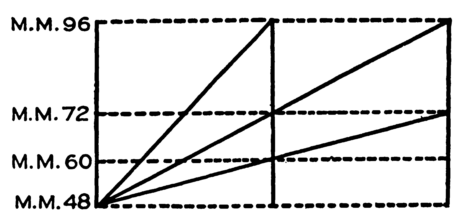
\includegraphics[width=\linewidth]{CowellPolytemp.png}
  \caption{Polytempic tempo transitions as illustrated by Henry Cowell
    in 1930. \textcircled{c} Cambridge University Press}
  \label{fig:cowell-polytemp}
\end{marginfigure}
While he was not a mathematician, Cowell did understand that there
were some unanswered complications surrounding simultaneous tempo
changes. While describing polytempic accelerations he says:
\begin{quotation}
``For practical purposes, care would have to be exercised in the use of
sliding tempo, in order to control relation between tones in a sliding
part with those in another part being played at the same time: a
composer would have to know, in other words, what tones in a part with
rising tempo would be struck simultaneously with other tones in a part
of, say, fixed tempo, and this from considerations of harmony. THere
would usually be no absolute coincidence, but the tones which would be
struck at approximately the same time could be calculated.''
\end{quotation}
It is possible to calculate exactly when tones in an accelerating
tempo will be struck. Probably the most important thing to understand
about the examples that Cowell gives, is that in the examples shown in
figure~\ref{fig:cowell-polytemp}, the linear tempo accelerations
rarely yield satisfactory results. The figure does not show how many
beats or measures elapse during the tempo acceleration, but with
linear acceleration only a few certain combinations will complete with
both tempi on a down beat.\sidenote{This is described in more detail
  in \autoref{ch:polytempic}.}

\subsection{Modernism and Rhythmic Complexity}
\label{sec:modern-rhythm-compl}
During the modernist period, many composers sought new ways to use
time and space as compositional elements. Polytempic music was
relatively unexplored. However, traditional music notation is not well
equipped to handle acceleration with precision. The convention is to
annotate the score with notes like \textit{ritardando} (gradually
slowing) and \textit{accelerando} (gradually accelerating) coupled
with traditional Italian tempo markings like \textit{adagio} (slow
stately, at ease) and \textit{allegro} (fast, quickly, bright) to
indicate tempo changes. Rates can be explicitly specified with an
M.M.\sidenote{In a musical score, M.M. stands for Maelzel's Metronome
  is accompanied by a number specifying the beats per minute.}
marking. While rates cam be quite specific, it is not realistic to
expect a performer to be able to follow an precise mathematical
acceleration. This did not stop modernist composers from finding
creative ways to notate surprisingly precise polytempic compositions
using only the conventional notation:
\begin{enumerate}
\item Groups of tuplets layered against a global tempo, as used by
  Henry Cowell (\textit{Quartet Romantic}, 1915-17), and Brian Fernyhough
  (\textit{Epicycle for Twenty Solo Strings}, 1968).
\item Polymeters are notated against a global tempo, and the value of
  a quarter note is the same in both sections, as in Elliott Carter's \textit{Double
    Concerto for Harpsichord and Piano with Two Chamber Orchestras}, 1961
  and George Crumb's \textit{Black Angels}, 1971.
\item Sections are notated without meter. Notes are positioned
  horizontally on the leger linearly according to their position in
  time. Conlon Nancarrow (\textit{Study No. 8 for Player Piano},
  1962), and Luciano Berio (\textit{Tempi Conceriati}, 1958-59).
\item The orchestra is divided into groups, and groups are given
  musical passages with varying tempi. The conductor cues groups to
  begin. Pierre Boulez, \textit{Rituel: In Memoriam Maderna} (1974).
\item One master conductor, directs the entrances of auxiliary
  conductors, who each have their own tempo, and direct orchestral
  sections. This approach was used by Brant Henry in \textit{Antiphony
    One for Symphony Orchestra Divided into 5 Separated Groups} (1953).
\end{enumerate}

\subsection{Charles Ives and The Unanswered Question}
\label{sec:charles-ives}
One composer did actually discover polytempic before \textit{New
  Musical Resources} was published. Charles Ives was an American
composer, who's works were largely overlooked during his lifetime. His
1908 composition \textit{The Unanswered Question} incorporates both
spatial and polytempic elements. In this piece, the string section is
positioned away from the stage, while the trumpet solist and woodwind
ensemble are on the stage. A dialogue between the trumpet, flutes, and
strings, is written into the music, with the trumpet repeatedly posing
a melodic question \textit{"The Perennial Question of
  Existence''}. Each question is answered by flute section. The first
response is synchronized with the trumpet part, but subsequent
responses accelerate, and intentionally desynchronize with the
soloist. Ives included a note at the beginning of the score which
describes the behavior of the ``answers'':
\begin{quotation}
This part need not be played in the exact time position indicated. It
is played in somewhat of an impromptu way; if there is no conductor,
one of the flute players may direct their playing.

The flutes will end their part approximately near the position
indicated in the string score; but in any case, "The Last Question"
should not be played by the trumpet until "The Silences" of the
strings in the distance have been heard for a measure or two. The
strings will continue their last chord for two measures or so after
the trumpet stops. If the strings shall have reached their last chord
before the trumpet plays "The Last Question", they will hold it
through and continue after, as suggested above.

"The Answers" may be played somewhat sooner after each "Question" than
indicated in the score, but "The Question" should be played no sooner
for that reason.
\end{quotation}
Ives gave the performers license over the temporal alignment, but he
made it clear the parts should not be played together. Following Ives,
other modernist composers also sought new ways to manipulate tempo and
meter. 

\subsection{Gruppen}
\label{sec:gruppen}
Ives' polytempic compositions from the first half of the 20th century
are somewhat of an exception. Polytempi was not widely explored until
well after \textit{New Musical Resources} was published. One famous
example is Karlheinz Stockhausen's \textit{Gruppen} for three
orchestras (1955-57). Parallel tempi that come in and out of
syncronicity is always a challenge with polytempic music, and
Stockhausen found an effective, if heavy-handed, solution. He
developed a system of discrete tempo changes. Each of the three
orchestras was to have it's own conductor. The conductor would listen
for a cue carefully written in to one of the other sections. That cue
would signal to the conductor to begin beating a silent measure at the
new tempo and prepare the new orchestra to begin playing.  Stockhausen
did not say that he was inspired by the \textit{New Musical Resources}
directly, but his famous essay \textit{How Time Passes} describes how
he chose the tempic ratios used in \textit{Gruppen}. Instead of basing
the tempo scales on simple pythagorean relationships, Stockhausen
based chose the relationships based on the $\sqrt[12]{2}$ ratio of
adjacent notes in equal tempered tuning.


\subsection{Conlon Nancarrow}
\label{sec:conlon-nancarrow}
Conlon Nancarrow is best known for his incredibly complex player piano
scores, and is recognized as one of the first composers to realize the
potential of technology to perform music beyond human capacity. Unlike
Stockhausen, Nancarrow did acknowledge the influence of Cowell's
\textit{New Musical Resources} on his own works. His compositions for
the player piano, beginning with \textit{Study for Player Piano
  No. 21}, did incorporate polytempic
accelerations\cite{Rao2005}. While some of Nancarrow's compositions do
feature many simultaneous tempi, (Study No. 37 features 12
simultaneous tempi)\cite{Greschak2003}, a rigorous mathematical
approach would be required for all 12 tempi to accelerate or
decelerate relative to each other, and synchronize at pre-determined
points. Interestingly, Nancarrow said in a 1977 interview that he was
originally interested in electronic music, but the player piano gave
him more temporal control.\cite{Amirkhanian1977}

% William Duckworth
% The Time Curve Preludes
% https://en.wikipedia.org/wiki/William_Duckworth_(composer)

\subsection{New Polytempi}
\label{sec:new-polytempi}
The many different approaches to polytempi in modernist music, all
have one thing in common: They all wrestle with syncronicity. Human
performers, are not naturally equipped to play simultaneous tempi, and
composers must find workarounds that make polytempic performance
accessible.

The examples described here exist in one or more of the following
categories:
\begin{enumerate}
\item The music may suggest, multiple tempi, but the beginning and end
  of the individual voices' measures align with each other.
\item The tempo changes are discrete, happening at either measure
  or beat divisions.
\item The tempo changes are somewhat flexible, and  the exact number of
  beats that elapse during a transition varies from one performance to
  another.
\item The tempo acceleration are linear, and align only at simple
  mathematical relationships.
\end{enumerate}
It is non-trivial to rigorously define parallel tempo curves that
accelerate and decelerate continuously relative to each other, and
come into syncronicity at strict predetermined musical points for all
voices. In \autoref{ch:polytempic}, we discuss how existing electronic
and acoustic music approaches this challenge, and derive a
mathematical solution that unlocks a previously inaccessible genre of
polytempic music.

\section{Amplified Spatial Music}
\label{sec:spatial-developments}
The evolution of polytempic music in the modernist period was
paralleled by innovation in the creation an performance of electronic
music. After World War II, new technology became available to
composers, and with the new technology, came new styles of music.
Pierre Schaeffer was among the first composers using electronic sounds
along together with acoustic ones.  He worked at the
Radiodiffusion-T\'{e}l\'{e}vision Fran\c{c}aise (RTF), where he helped
to pioneer early practices in musique concr\`{e}te. With the help of
younger composer Pierre Henry, he as also among the first composing
spatialized pre-recorded sound. The pair collaborated on a piece
called \textit{Symphonie pour un Homme Seul} (Symphony for One Man
Alone, 1950). For this piece they created an tetrahedral loudspeaker
arrangement, and a rather dramatic interface, they called the
\textit{Pupitre d'espace}, shown in figure~\ref{fig:schaeffer}. Large
hoops on the device had inductive coils that sensed the user's hand
position, and controlled the signal routing to the
loudspeakers.\cite{Holm2008}
\begin{marginfigure}
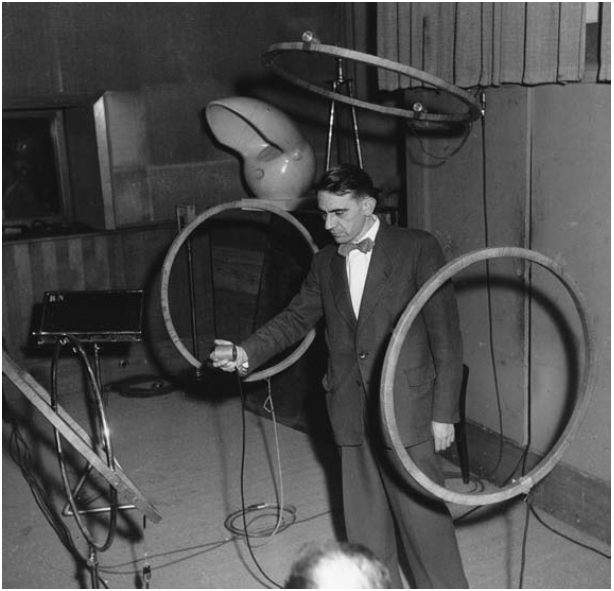
\includegraphics{Schaeffer.png}
\caption{Pierre Schaeffer with the \textit{Pupitre d'espace} in
  1951. \textcircled{c} Ina/Maurice Lecardent, Ina GRM Archives}
\label{fig:schaeffer}
\end{marginfigure}


\subsection{Gesang der J\"{u}nglinge}
The success of Schaeffer's music at the RTF attracted the attention of
other composers interested in electronic music. Among them was
Karlheinz Stockhausen. Stockhausen came to RTF, and composed just one
2-track etude in 1952 before returning to West Germany where he
continued to compose orchestral and electronic works. His practice led
to the composition of what is widely regarded as the first masterpiece
of electronic music: \textit{Gesang der J\"{u}nglinge} (Song of the
Youths, 1955-56), which was also the first multichannel pre-recorded
composition to be performed in a concert setting with multiple
loudspeaker placed around the audience,\cite{Grout2006}. 

The piece stands out by the many aspects in which it is both
evolutionary and revolutionary when juxtaposed with the other
electronic compositions of the time; the delicate blending of the
voice with electronics, and the creative editing of the voice being
two examples. It has been extensively analyzed and reviewed in
literature,\cite{Decroupet1998,Metzer2004,Miller2009} however the
exact strategy for the spatialization of sound in the original
four-channel performance remains somewhat ambiguous. From interviews,
and essays with Stockhausen, we can gather some insight into his
process. In 1955, the year when Stockhausen began work
on he published an essay on his serial technique. An English
translation finishes with the following comment:
\begin{quotation}
``By regulating the positions of the sources of sound it will be
possible for the first time to appreciate aesthetically the universal
realisation of our integral serial technique.''\cite{Stockhausen1955}
\end{quotation}
In an interview published in 1974, he made the following comment the
subject of sound positioning in \textit{Gesang der J\"{u}nglinge}:
\begin{quotation}
  ``The speed of the sound, by which one sound jumps from one speaker to
  another, now became as important as pitch once was. And I began to
  think in intervals of space, just as I think in intervals of pitch
  or durations. I think in chords of space.''\cite{Stockhausen1974}
\end{quotation}
A side-effect of serialism is discouraging the uneven distribution of
a musical parameter. With this in mind, spatialization is a very
natural target for serialism. Given the added creative flexibility of
surround sound, it reasonable to search for ways to take full
advantage of the new dimension, without favoring any particular
direction or loudspeaker.

\begin{figure}
  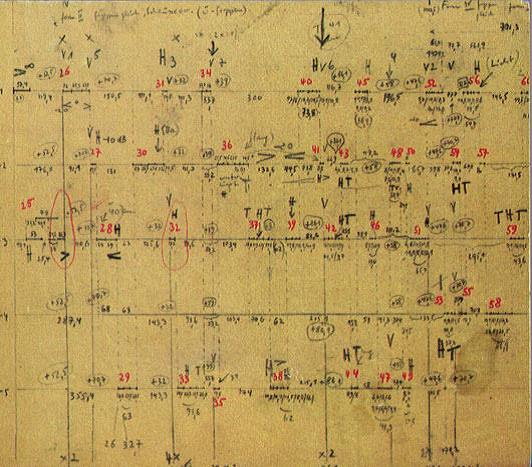
\includegraphics{Gesang.jpg}
  \caption{Excerpt from the \textit{Gesang der J\"{u}nglinge}
    manuscript. \textcircled{c}~www.karlheinzstockhausen.org}
  \label{fig:schaeffer-score}
\end{figure}

\subsection{Advances in Surround Panning}
\label{sec:advanc-surr-pann}
For his next four-track tape composition, \textit{Kontakte}
(1958-60), Stockhausen devised a new technology that made it quite
simple to continuously pan sounds between the speakers, orbiting the
listener. He used a rotating speaker on a turntable, surrounded by
four equally spaced microphones. Stockhausen continued to feature
spatialization prominently in both acoustic, and electronic work.  His
major orchestral compositions, \textit{Gruppen} (1955-57, described in
section~\ref{sec:gruppen}) and \textit{Carr\'{e}} (for four orchestra
and four choirs, 1959-60) both prominently feature spatialization.

Throughout the rest of the century, advances in technology enabled new
performances with more speakers, and more complex spatial
possibilities. The Vortex multimedia program at the Morrison
Planetarium in San Francisco (1957-59) featured 40 loudspekaers, with
surround sound panning facilitated by a custom rotary console, and
featured works by Stockhausen, Vladimir Ussachevsky, Toru Takemitsu,
and Luciano Berio. The planetarium featured synchronized lighting,
which became a hallmark of major surround sound productions of the
time. The Philips Pavilion at the 1958 Brussels Worlds' Fair used a
custom sequncser hooked up to a telephone switcher to pan sounds
between over 300 speakers (more in
section~\ref{sec:philips-pavilion-1}).  John Chowning’s
\textit{Turenas}, (1972) simulated amplitude changes and doppler shift
pitch modulations of sound objects movement as a compositional
element.\cite{Chowning2011} The West German pavilion at Expo 70 in
Osaka, Japan, included a dome 28 meters in diameter, five hours of
music composed by Stockhausen, and 20 soloist musicians. Stockhausen
``performed'' the live three-dimensional spatialization from a custom
console near the center of the dome (figure~\ref{stockhausen-expo}).
\begin{figure}
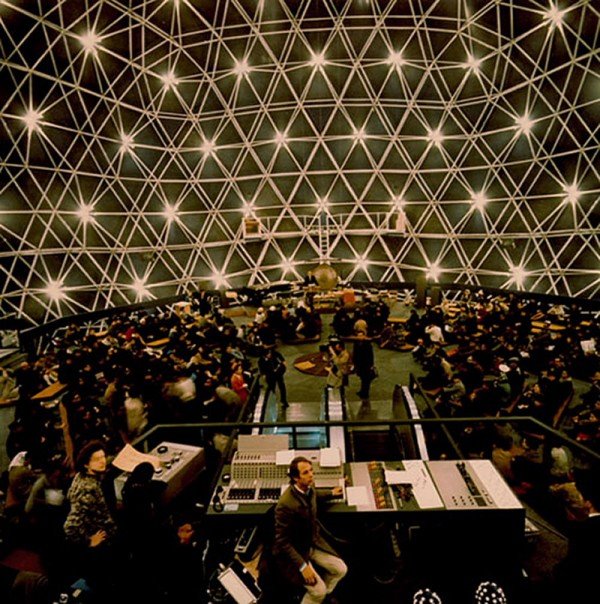
\includegraphics{Expo70.jpg}
\caption{Inside the West Greman pavillion at Expo 70. Osaka, 1970.}
\label{fig:stockhausen-expo}
\end{figure}
The West German dome was not the only massive spatialized sound
installation at Expo 70. Iannis Xenakis, the mastermind behind the
1958 Philips Pavilion in Brussels, was aslo presenting his 12-channel
tape composition, \textit{Hibiki Hana Ma} at the Japanese Steel
Pavilion through 800 speakers positioned around the audience,
overhead, and underneath the seats. 

%\TODO{Ambisonics, Commercial options like Dolby}

\subsection{Evolution Of Electronic Composition}
\label{sec:evolution-of-electronic-composition}
\textit{Gesang der J\"{u}nglinge} may have been the first masterpiece
of electronic music, but the techniques that were developed at the RTF
studios were quickly spreading Another composer who came was drawn to
RTF (where musique concr\`{e}te was first conceived by Pierre
Schaeffer) was Pierre Boulez. However, Boulez was generally
unsatisfied with his early electronic compositions, and frustrated by
the equipment required to make electronic music. Despite his general
distaste for electronic music composition, Boulez was approached by
the French President, Georges Pompidou, in 1970 and asked to found
institution dedicated to the research of modern musical practice. The
center opened in 1977 with Boulez at the head. In a 1993 interview,
Boulez described how he directed the efforts of the lab:
\begin{quotation}
  ``Back in the 1950s, when you were recording sounds on tape and using
  them in a concert, you were merely following the tape, which became
  very detrimental to the performance. So I pushed the research at
  IRCAM to examine the use of live electronics, where the computer is
  created for the concert situation, instantly responding to your
  actions. The system's language also became easier to follow; I
  remember when I tried to learn the electronics, it was all figures,
  figures, figures. These meant nothing at all to the musician. If you
  have to work in hertz and not notes, and then wait half an hour to
  process the sounds, you get completely discouraged. My goal was so
  that the musician could sketch his ideas very rapidly, with
  instantaneous sound and graphical notation. The use of computers
  finally brought electronics down to the level of understanding for
  composers. I feel very responsible for that change.''\cite{Carvin1993}
\end{quotation}
Boulez' first major composition that took advantage of the resources
at IRCAM was \textit{R\'{e}pons} which premiered at the Donaueschingen
Festival in Germany in 1981 (allthough Boulez continued to revise it
until 1984). The piece balances 24 acoustic performers with pre-recorded material
and live processing with spatialization over a ring of 38 loudspeakers
8. The audience sits in a circle surrounding the orchestra, while six
of the acoustic instrumentalists are spaced around the outside of the
audience. Boulez was certainly not the first composer to
mix elextronics with acoustic performers, (Milton Babbitt's 1964
\textit{Philomel} is a much earler example), but \textit{R\'{e}pons}
does mark a certain maturity of maturity of the form.

% Janet Cardif? 40 part motet wasn't until 2001
% \TODO{Berio, Boulez (repons), Stockhausen (Gesang der Junglinge), etc}

\section{Iannis Xenakis}
\label{sec:iannis-xenakis}
The projects in this thesis build on the work and ideas of Iannis
Xenakis. Xenakis studied music and engineering at the Polytechnic
Institute in Athens, Greece. By 1948, he had graduated from the
university and moved to France where he began working for the French
architect, Le Corbusier. The job put his engineering skills to use,
but Xenakis also wanted to continue studying and writing music. While
searching for a music mentor, he approached Oliver Messiaen, and asked
for advice on whether he should study harmony or
counterpoint. Messiaen was a prolific French composer known for
rhythmic complexity. He was also regarded as a fantastic music
teacher, and his students included Stockhausen, Boulez.  Messiaen
later described his conversation with Xenakis:
\begin{quotation}``I think one should study harmony and
  counterpoint. But this was a man so much out of the ordinary that I
  said: No, you are almost 30, you have the good fortune of being
  Greek, of being an architect and having studied special
  mathematics. Take advantage of these things. Do them in your
  music.''\cite{Service2013}
\end{quotation}
In essence, Messiaen was rejecting Xenakis as a student, but we can
see how Xenakis ultimately drew from his disparate skills in his
compositions. The score for his 1945 composition \textit{Metastasis}
(figure~\ref{fig:metastasis}) resembles an architectural blueprint as
much as it does a musical score.

\begin{figure*}[h]
  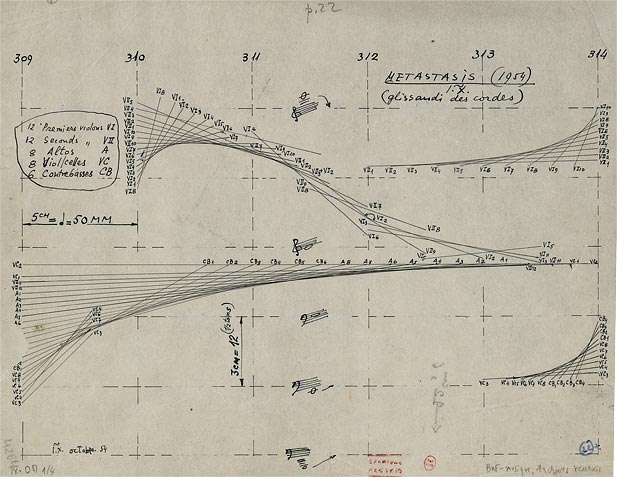
\includegraphics[width=\linewidth]{XenakisMetastasis.jpg}
  \caption{Excerpt from Iannis Xenakis' composition,
    \textit{Metastasis} (1954), measures 309-314. This score in this
    image was then transcribed to sheet music for the orchestral
    performance.}
  \label{fig:metastasis}
\end{figure*}

\subsection{The Philips Pavilion}
\label{sec:philips-pavilion-1}
\begin{figure}[h]
  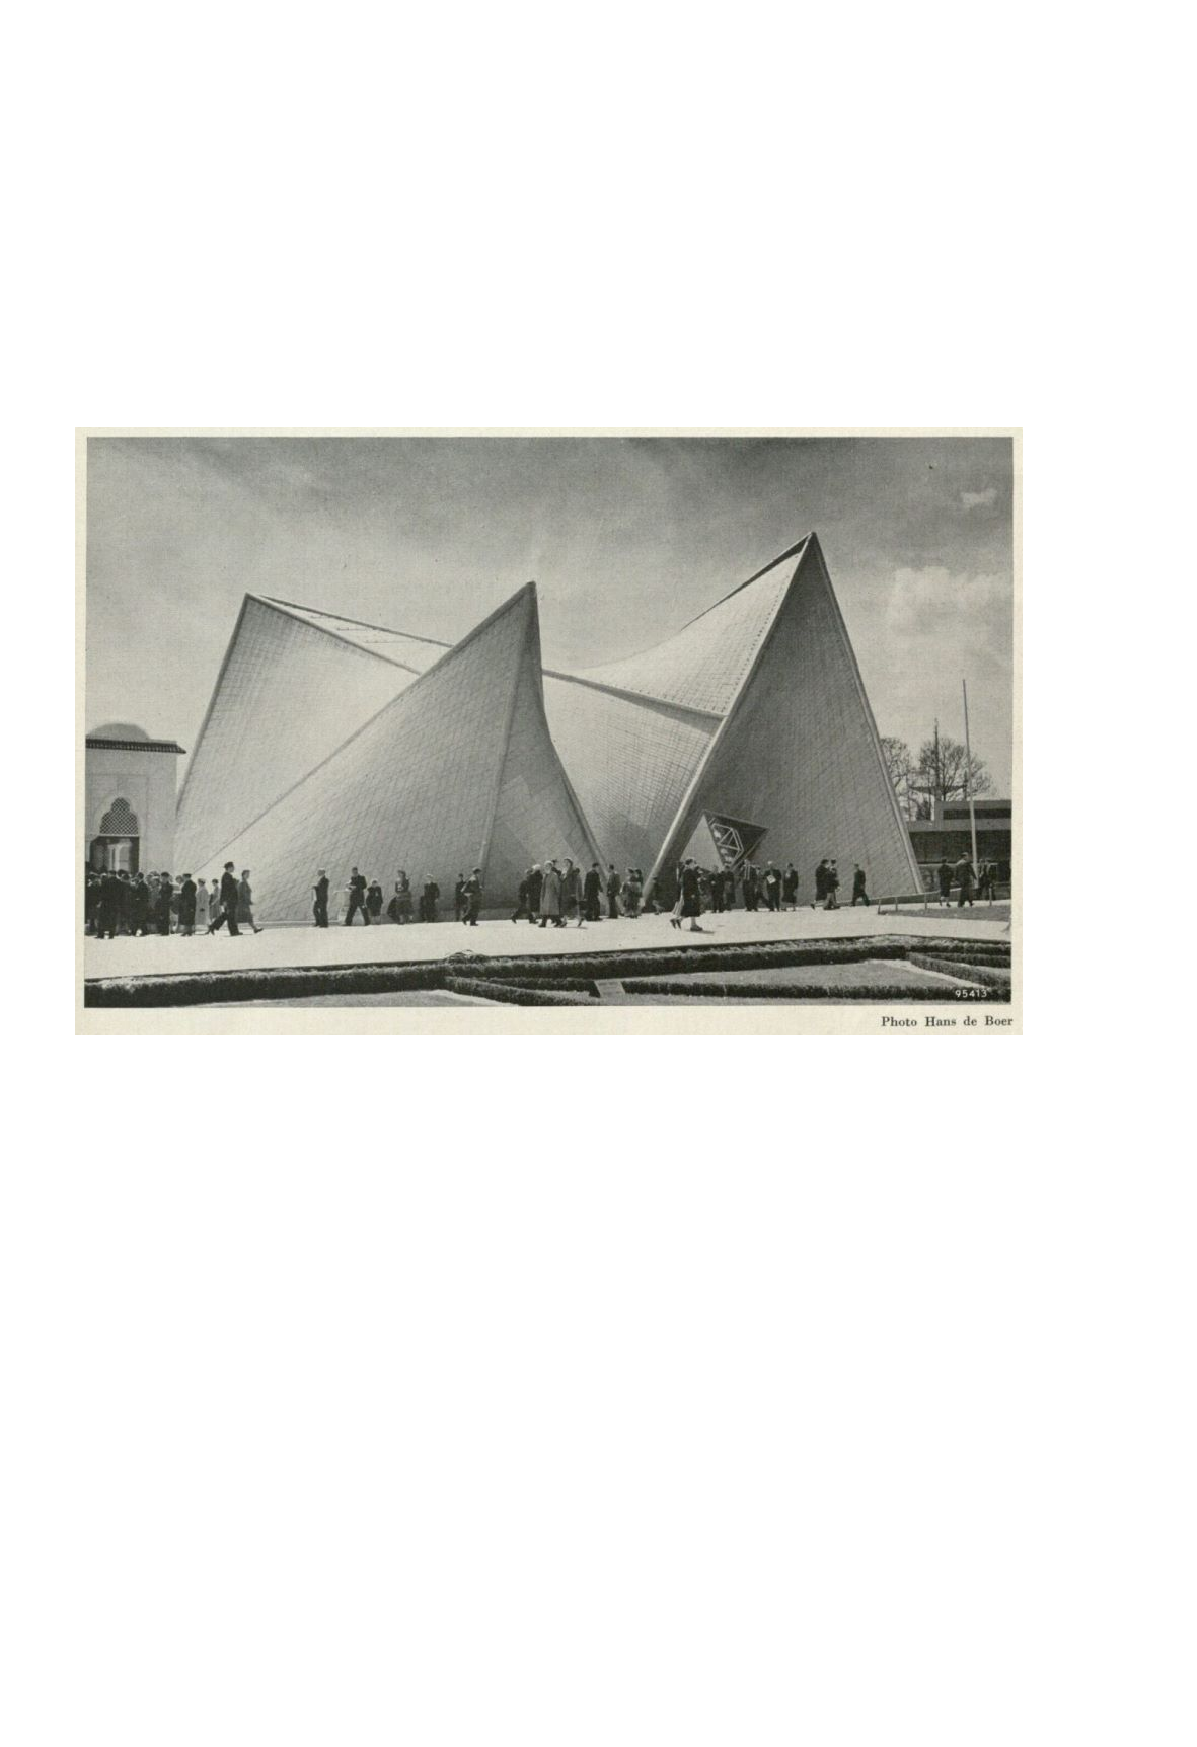
\includegraphics[width=\linewidth]{PhilipsPavilion-TechnicalReview-00.pdf}
  \caption{The Philips Pavilion at the 1958 Brussels World Fair as
    shown in Volume 20 of the \textit{Philips Technical Review}, 1959.}
  \label{fig:philips-pavilion-photo}
\end{figure}
In 1956, Le Corbusier was approached by Louis Kalff (Artistic Director
for the Philips corporation) and asked to build a pavilion for the
1958 World's Fair in Brussels. The pavilion was to showcase the sound
and lighting potential of Philips' technologies. Le Corbusier
immediately accepted, saying:
\begin{quotation}
  ``I will not make a pavilion for you but an Electronic Poem and a
  vessel containing the poem; light, color image, rhythm and sound
  joined together in an organic synthesis.''\cite{Lopez2011} 
\end{quotation}
The final product lived up to Le Corbusier's initial description. It
included:\cite{Lombardo2009}
\begin{enumerate}
\item A concrete pavilion, designed by architect and composer Iannis
  Xenakis
\item \textit{Interlude Sonoire} (later renamed \textit{Concret PH}), a
  tape music composition by Iannis Xenakis, approximately 2 minutes
  long, played between performances, while one audience left the
  pavilion and the next audience arrived
\item \textit{Po\`{e}me \'{E}lectronique}, a three channel, 8 minute
  tape music composition by composer Edgard Var\`{e}se
\item A system for spatialized audio across more than 350 loudspeakers
  distributed throughout the pavilion
\item An assortment of colored lighting effects, designed by Le Corbusier in
  collaboration with Philips' art director, Louis Kalff
\item Video consisting mostly of black and white still images,
  projected on two walls inside the pavilion
\item A system for synchronizing playback of audio and video,
  with light effects and audio spatialization throughout the
  experience
\end{enumerate} 

\paragraph{Role of Iannis Xenakis} During the initial design stage, Le
Corbusier decided that the shape of the pavilion should resemble a
stomach, with the audience entering through one entrance and exiting
out another. He completed initial sketches of the pavilion layout and
then delegated the remainder of the design to
Xenakis.\cite{Clarke2012}

The architectural evolution of the pavilion from Le Corbusier's early
designs (figure~\ref{fig:le-corbusier-sketch}) to Xenakis' iterations
(figure~\ref{fig:xenakis-draw}), illustrates the profound impact that
Xenakis had on the project. An article in the \textit{Philips
  Technical Review}\cite{philips1958} gives a wonderfully detailed
account of Xenakis' process in restructuring the design:\sidenote{\TODO{Clean this section.}}
\begin{enumerate}
\item Xenakis was aware that parallel walls and concave spherical
  walls would both negatively impact audio perceptibility due to repeated
  or localized acoustic reflections.
\item To accommodate musical purpose of the space he decided to
  explore surfaces with varying curvature...
\item 
  \begin{marginfigure}
    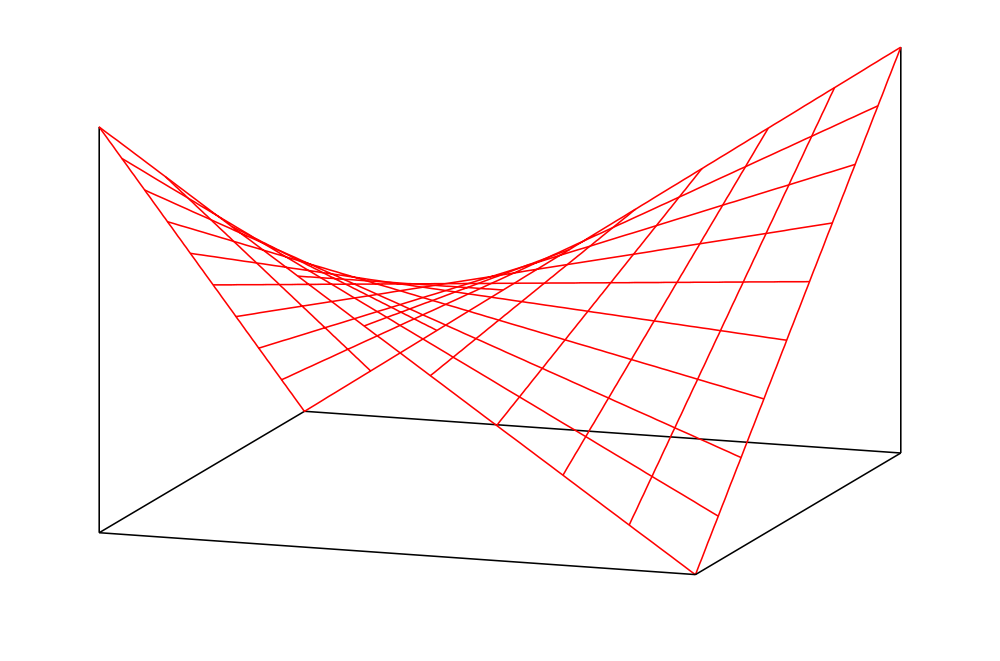
\includegraphics{hyperbolic-paraboloid}
    \caption{A ruled surface. For a surface to be considered ``ruled''
      every point on the surface must be on a straight line, and that
      line must lie on the surface. In Xenakis' time, ruled surfaces
      were useful in architecture, because they simplified the
      construction of curved surfaces by using straight beams.}
    \label{fig:ruled-surface}
  \end{marginfigure}...leading him to consider ruled surfaces such as
  the conoid and hyperbolic paraboloid. 
\end{enumerate}
Through this process, we see Xenakis utilizing the skills that he
learned at the Polytechnic Institute and continued to develop while
working with Le Corbusier. He also understood the mathematical
formation of the ruled surfaces that make up the structure. These
surfaces even look familiar to the Metastasis score
(figure~\ref{fig:metastasis}). In his 1963 book, \textit{Formalized
  Music}, Xenakis explicitly states that the Philips Pavilion was
inspired by his work on \textit{Metastasis}.

\begin{figure*}[]
  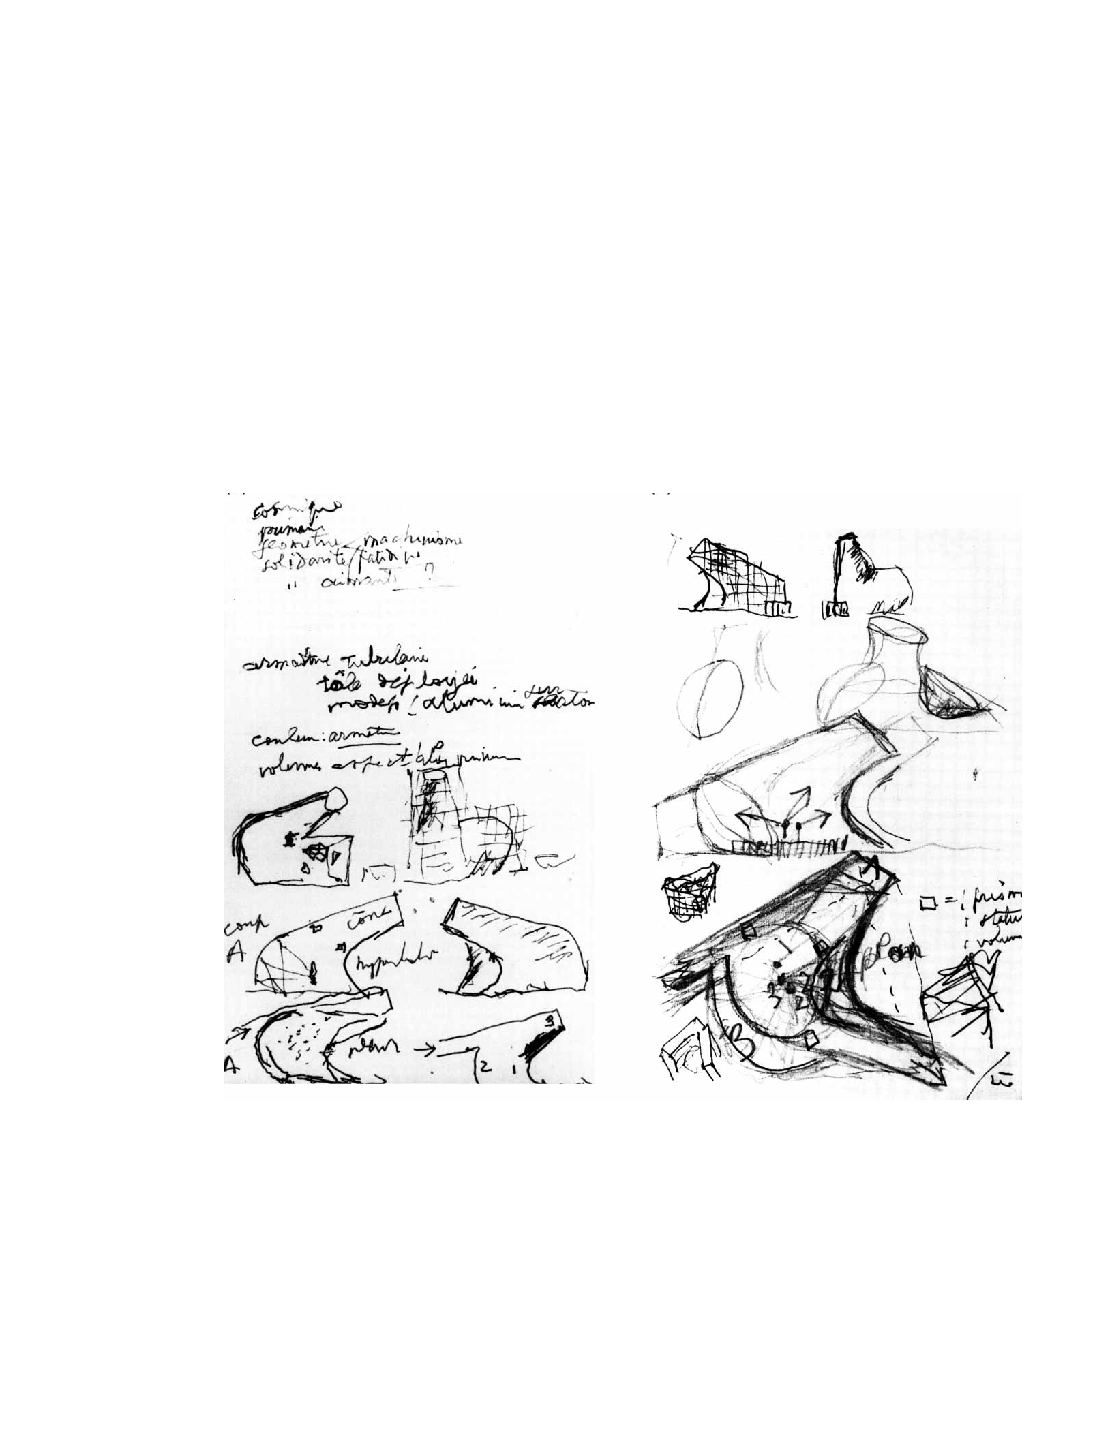
\includegraphics[width=\linewidth]{LeCorbusierDraw.pdf}
  \caption{Le Corbusier's design sketches for the Philips Pavilion,
    September \textendash{} October, 1956 (\textcircled{c} 2012
    Artists Rights Society, New York/ADAGP, Paris/FLC)}
  \label{fig:le-corbusier-sketch}
\end{figure*}

\begin{figure*}[h]
  % XenakisSketch.pdf or PhilipsDrawings.jpg
  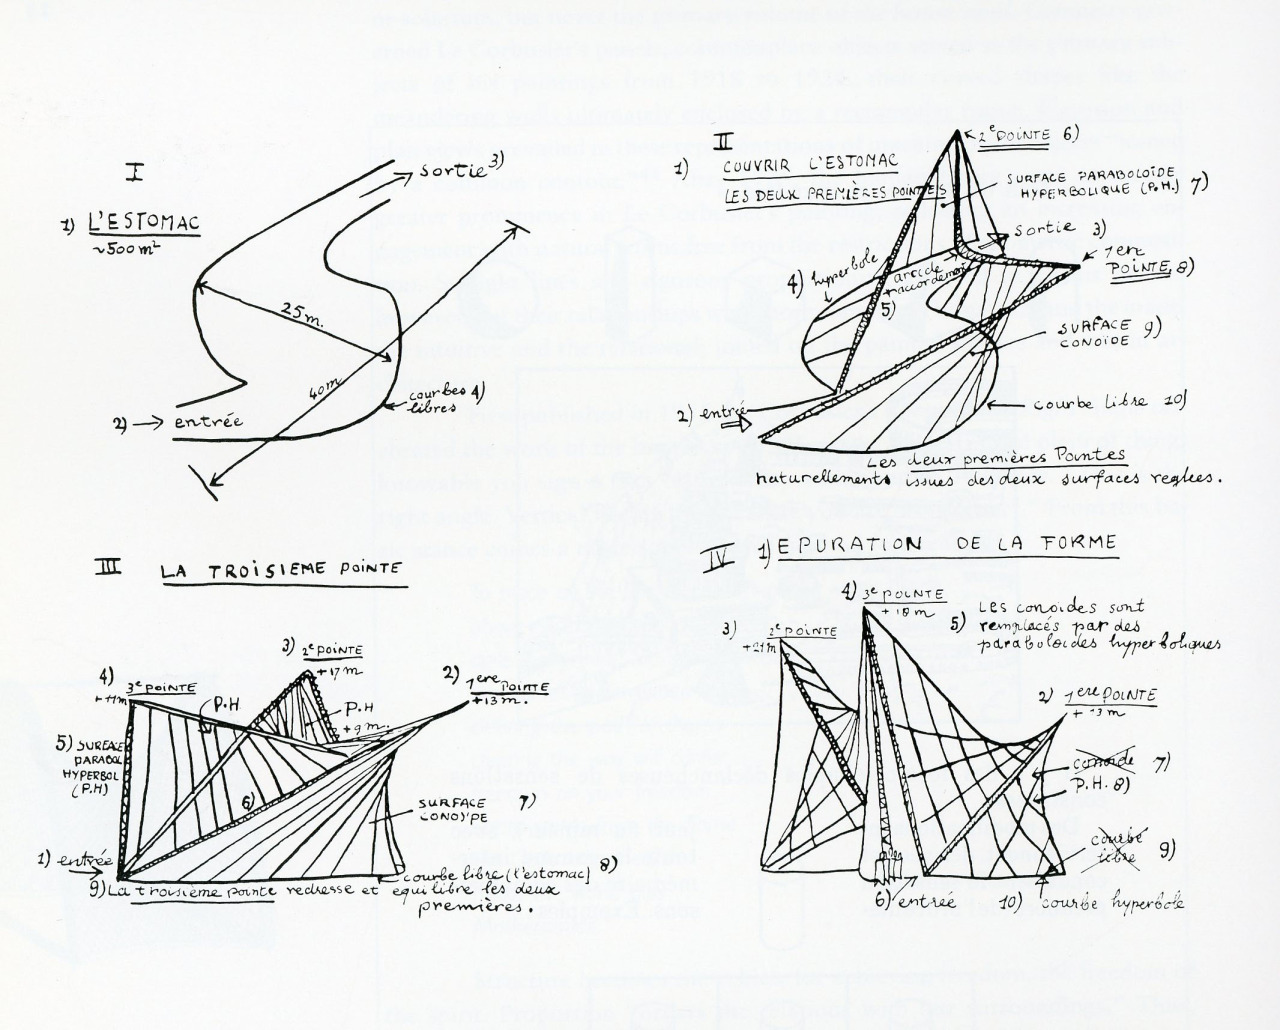
\includegraphics[]{PhilipsDrawings.jpg}
  \caption{Xenakis' early drawings of the Philips Pavilion as
    documented in volume 20 of the \textit{Philips Technical Review}.}
  \label{fig:xenakis-draw}
\end{figure*}

\section{Architecture and Music in Space and Time}
\label{sec:introduction-conclusion}

In \textit{Formalized Music}\cite{xenakis1992formalized}, Xenakis
describes how developments in music theory mimic equivalent
developments in philosophy, mathematics, and the sciences. Plato, for
example, believed that all events transpire as determined by cause and
effect. While Plato and Aristotle both described causality in their
writing, it was not until the 17th century that controlled experiments
and mathematics corroborated the theory.\sidenote{In 1687, Isaac
  Newton published \textit{Philosophi\ae{} Naturalis Principia
    Mathematica} (\textit{Mathematical Principles of Natural
    Philosophy}), in which he compiled the 3 laws of motion that set
  the foundation for the study of \emph{classical mechanics}.}
Similarly, music theory has historically employed causal rules to
describe counterpoint, tonality, and harmonic movement.\sidenote{\TODO{Add example}}

Causality was largely used to describe physical phenomena until the
19th century when statistical theories in physics began to include
probabilistic notions.\sidenote{The Maxwell-Boltzmann distribution,
  which was first derived by James Clerk Maxwell in 1860, describes
  the probability distribution for the speed of a particle within an
  idealized gas. For more see
  \url{http://plato.stanford.edu/entries/statphys-statmech/}} Xenakis
noticed that more contemporary fields like \emph{probability theory}
generalize and expand on the antecedent theories of causality. Xenakis
thought that music composition should naturally follow the progression
that physics did, with music theory generalizing and expanding on
causal rules that had existed previously. Indeed, starting in the late
19th century and early 20th century, composers like Strauss and
Debussy began to bend the existing rules of music theory, composing
music that branched away from the causal and tonal theories of the
time. With the rise of serialism\sidenote{Serialism is a technique for
  musical composition in which instances of musical elements (such as
  pitch, dynamics, or rhythm), are given numerical values. Sequences
  built from the values are ordered, repeated and manipulated
  throughout the composition.}  and indeterminate music\sidenote{In
  music, indeterminacy refers to the use of chance (such as rolling
  dice or flipping coins) as part of the compositional process.},
composers such as Stockhausen, Boulez, John Cage, Aaron Copland, and
B\'{e}la Bart\'{o}k began to use probability and chance in
composition, the same way that physicists were using probability to
describe the material world. 

To Xenakis' mind, serial music was no less causal than the music it
intended to supersede. He described serial music as embodying
``virtually absolute determinism.''\cite{xenakis1992formalized}
Xenakis saw music theory as a sub-set of mathematics and algebra:
While musicians have a different vocabulary, they also use
mathematical principles to describe and compose music. Because Xenakis
understood mathematics as well as music, he was able to identify how
even in serialism and indeterminate music, composers were only
utilizing a small subset of algebraic theory. In his own music,
Xenakis wanted to generalize and expand the causal framework that
musicians and theorists had been using to compose and understand
music, paralleling similar developments in physics and
mathematics. As a reference to \emph{chance}, or \emph{stochos},
Xenakis coined the term \emph{stochastic music} to describe his
development.\sidenote{\TODO{Clarify}}

Xenakis' book, \textit{Formalized Music} gives a verbose explanation
of stochastic music. Some authors have interpreted his description
more explicitly. In \textit{Audible Design}, Trevor Wishart describes
the stochastic process used to compose stochastic music as:
\begin{quotation}
  ``A process in which the probabilities of proceeding from one state,
  or set of states, to another, is defined. The temporal evolution of
  the process is therefore governed by a kind of weighted randomness,
  which can be chosen to give anything from an entirely determined
  outcome, to an entirely unpredictable one.''\cite{Wishart1994}
\end{quotation}
% It could be that the lack of a single clear definition by Xenakis is
% the reason that few composers today identify their work as stochastic
% music.

\paragraph{Xenakis' Reflection} In the Spring of 1976, while defending
his doctoral thesis at the University of Paris, Xenakis emphasized the
relevance of seemingly unrelated disciplines to the creative process. A
translation of his defense includes this statement:
\begin{quotation}
  ``The artist-conceptor will have to be knowledgeable and inventive
  in such varied domains as mathematics, logic, physics, chemistry,
  biology, genetics, paleontology (for the evolution of forms), the
  human sciences, and history; in short, a sort of
  \emph{universality}, but one based upon, guided by and oriented
  toward forms and architectures.''\cite{russolo1986art}
\end{quotation}
From Xenakis' drawings we can deduce that he used the same tools,
skills, and philosophy to imagine and conceive both music and
architecture. His approach elevated both forms and blurred the distinction
between the two. Perhaps if we had kept using pen and paper to design
buildings and write music, the reality today would be closer to the
ideal that he imagined. 

As the ideas that inspired Xenakis and other progressive 20th century
composers were taking root in contemporary music, the culture of
artistic form and composition was already beginning the transition
into the digital domain. There is no reason why digital tools cannot
favor stochastic processes to linearity; there is no reason why
digital tools cannot treat music and architecture as equals. However,
even today, software for composing music still favors static pitches
to glissandi; software for architectural design still favors corners
to curves. Most importantly, the software skills that we use to design
and manipulate space, and the skills that we use to compose music,
mutually exclude each other.

This is where the projects described here make a contribution.  By
drawing from music, mathematics, computer science, acoustics, audio
engineering and mixing, sound reinforcement, multimedia production,
and live performance, we can create tools that allow us to
indiscriminately compose with space and sound.

%%% Local Variables:
%%% mode: latex
%%% TeX-master: "CharlesHolbrow_MAS_Thesis"
%%% End:
